\documentclass[12pt,a4paper,english]{article}
\usepackage[latin1]{inputenc}
\usepackage[T1]{fontenc}
\usepackage[english]{babel}
\usepackage{graphicx}
\usepackage{fancyhdr}
\usepackage{geometry}
\usepackage{helvet}
%\usepackage{scrpage2}
\usepackage{subfigure}
\usepackage{epsfig}
\usepackage{textcomp} % degree celsius
\usepackage{natbib}
\usepackage{afterpage}
\usepackage{amssymb}
\usepackage{subfigure}
\usepackage{babel}
\usepackage{float}
\usepackage{tabularx}
\usepackage{multirow}
%\usepackage{pyenchant}
\usepackage[footnotesize,sl]{caption}
\usepackage{pdfpages}
\usepackage{enumerate}

\geometry{verbose,a4paper,tmargin=25mm,bmargin=17mm,lmargin=17mm,rmargin=17mm}

\setcounter{secnumdepth}{4} 
 


\begin{document}

\bibliographystyle{ams}

\thispagestyle{empty}

\begin{figure}[!ht]
\begin{center}
\includegraphics*[height=29.6mm,width=183mm]{Figs/Topp_report.png}
\end{center}
\end{figure}

\begin{flushright}
{\bf \fontfamily{phv} no. 08/2012 \\ Climate}
\end{flushright}

\vspace{8mm}

\begin{center}

{\LARGE \bf Estimation of extreme precipitation in Norway and a summary of the state-of-the-art}

\vspace{6mm}

{\large \bf Anita Verpe Dyrrdal}

\end{center}

\vspace{10mm}

\begin{figure}[htbp]
\begin{center}

\epsfig{file=Figs/rainfall.jpg, width = 0.65\linewidth,clip=} 
\end{center}\end{figure}

%\begin{figure}[htbp]
%\begin{center}
%
\includegraphics[width = \linewidth]{Figs/rainfall.pdf} 
%\end{center}
%\caption[Map]{\label{data:fig2}Catchments}
%\end{figure}

\clearpage
\newpage

\thispagestyle{empty}

\fontfamily{ptm}\selectfont

%\includepdf[pages=-]{figs/signed.pdf} 

\begin{figure*}[t]
\centering
\includegraphics[width=1.0\textwidth]{signed.pdf}
\end{figure*}

\newpage

\begin{table}[!ht]
\begin{tabular}[c]{lr}
\includegraphics*[height=17mm]{Figs/metesort.png} & \hspace{20mm} {\Huge \bf \em \fontfamily{phv}\selectfont report} \\
\end{tabular}
\end{table}


\setlength{\unitlength}{1mm}  %Needed for picture environment

\begin{table}[!ht]
\vspace{-3mm}
\begin{tabular}[t]{|p{130mm}|p{43mm}|} \hline

{\bf Title}                  & {\bf Date}               \\ 
Estimation of extreme precipitation in Norway and a summary of the state-of-the-art        
      
                             & \today                   \\ \hline
{\bf Section}                & {\bf Report no.}         \\ 
Climate                      & no.08/2012              \\ \hline
{\bf Author(s)}                 & {\bf Classification}     \\ 
Anita Verpe Dyrrdal                     & \begin{picture}(20,4)(-2,-1.0)
                               \put (0,0){\circle*{4}}
                               \put (7,0){\makebox(0,0){Free}}
                               \put (15,0){\circle{4}}
                               \put (27,0){\makebox(0,0){Restricted}}
                               \end{picture}            \\
                               \cline{2-2}
                             & {\bf ISSN 1503-8025}     \\
                               \cline{2-2}
                             & {\bf e-ISSN 1503-8025}     \\ \hline
{\bf Client(s)}              & {\bf Client's reference} \\ 
Norwegian Water Resources and Energy Directorate (NVE), Jernbaneverket, Statens veivesen                  &             \\ \hline
\end{tabular}
\begin{tabular}[t]{|p{177.25mm}|} \hline
{\bf Abstract} \\
Estimates of extreme precipitation in points and larger areas are of great importance. They are applied in the planning of infrastructure such as water dams and transportation facilities, and also in forecasting and flood frequency estimation. In this work we aim to provide a summary of existing methodology applied at met.no as well as a description of the procedure for estimating extreme precipitation in station sites and catchments in Norway. This methodology is found to be laborious, outdated, and associated with inconsistency as it introduces a number of subjective measures. International research on the area and methods applied in a number of countries are also presented, and a proposed method using a national gridded dataset is introduced.                                          \\ 
  

                              
\\ \hline

{\bf Keywords} \\
Extreme precipitation, areal precipitation                                          \\ 



   \\ 
                                                        \\ \hline

\end{tabular}

\begin{tabular}[t]{|cc|}\hline

{\bf Disciplinary signature}  & {\bf Responsible signature} \\ 
                             &                             \\
                             &                             \\
                             &                             \\
\line(1,0){70}               & \line(1,0){70}              \\ 
Torill Engen-Skaugen          & {\O}ystein Hov              \\
\hspace{86.5mm}              & \hspace{86.5mm}             \\ \hline

\end{tabular}

\begin{tabular}[t]{p{23mm}p{30mm}p{17mm}p{17mm}p{30mm}p{18mm}p{16mm}}

 \begin{minipage}[l]{23mm} \tiny {\bf Postal address}\\  \tiny P.O Box 43 Blindern \\ \tiny N-0313 OSLO \\ \tiny Norway  
 \end{minipage} & 
 \begin{minipage}[l]{30mm} \tiny {\bf Office}        \\  \tiny Niels Henrik Abels vei 40            
 \end{minipage} &
 \begin{minipage}[l]{17mm} \tiny {\bf Telephone}     \\  \tiny +47 2296 3000 
 \end{minipage} & 
 \begin{minipage}[l]{17mm} \tiny {\bf Telefax}       \\  \tiny +47 2296 3050   
 \end{minipage} & 
 \begin{minipage}[l]{30mm} \tiny {\bf e-mail:}  met.inst@met.no  \\  \tiny {\bf Internet:}  met.no   
 \end{minipage} & 
 \begin{minipage}[l]{18mm} \tiny {\bf Bank account}  \\  \tiny 7694 05 00601   
 \end{minipage} & 
 \begin{minipage}[l]{16mm} \tiny {\bf Swift code}    \\  \tiny DNBANOKK       
 \end{minipage} 
 \tabularnewline[1mm]
  
\end{tabular}
\end{table}

\clearpage

{\renewcommand{\baselinestretch}{1.0}
\small

\tableofcontents
}

\clearpage


\section{Introduction}

Floods in small catchments and urban areas result in large economic loss every year, and can be a threat to life and property. A major trigger of floods in urban areas and regions of steep topography is intense and/or prolonged rainfall, particularly in combination with snow melt. The Norwegian Water Resources and Energy Directorate (NVE) has estimated the average annual cost of flood damage in Norway to be about 200 million NOK. Over-design of reservoir storage capacities can represent unnecessary expenses on a national level, while under-design can lead to losses associated with damage and in the worst case, loss of life. The direct or indirect damage on important infrastructure such as transport lines, caused by extreme precipitation, also requires large resources every year. Thus, in the light of the previously mentioned challenges, there is a great need for accurate estimates of extreme precipitation for current and future climate in Norway.

According to \cite{HanssenBaueretal2009} an increase in mean precipitation is observed in the entire country the last century, particularly since the end of the 1970s, and this trend is projected to continue in the future. The same report presents projections of increasing frequency and intensity of extreme precipitation events. In addition the latest special report of the Intergovernmental Panel on Climate Change, regarding extreme events \citep{SREX2012}, concluded that high extremes of precipitation are likely to increase in frequency. With a changing climate the intensity of rainfall induced floods are expected to increase as well, while higher temperatures probably lead to a shift towards earlier spring floods and increased possibility for late autumn,- and winter floods \citep{Wilsonetal2010, HanssenBaueretal2009, Hisdaletal2006}.

Extreme precipitation is usually presented as values with long return periods. In the dam safety regulations for Norway (NVE, 2009) it is stated that dams, depending on the dam category, should handle a design inflow with a 500-1000 year return period. Precipitation with 1000 year return period (P1000) and the probable maximum precipitation (PMP) is also applied in flood estimation in Norway, where PMP is defined as the theoretical maximum precipitation for a given duration under modern meteorological conditions \citep{WMO2009a}. PMP is used to estimate the probable maximum flood (PMF), which in turn is used in planning and design of hydraulic structures. Authorities for transport and urban planning are more concerned with short and intense precipitation with return periods of 5 to several hundred years. Extreme value theory deals with modeling the upper or lower tail of a distribution. In accordance with the definition of extreme there exist few or no observations of the tail, requiring extrapolation of observed values. Extrapolation is a challenging task which needs to be handled carefully, as the distribution of the very extreme events might differ from that of the less extreme events. The procedure of extrapolation is to fit the empirical distribution of the tail to a theoretical model and extend this to longer return periods. The most established models are the Generalized extreme value (GEV) distribution and the Generalize Pareto distribution (GPD) \citep{Coles2001}. The latter uses a peak-over-threshold approach. The GEV consists of three distributions differing by the width of the tail; Gumbel (EV1), Fr\'echet (EV2), and Weibull (EV3). \cite{Willeke1980} presented four common myths in hydrology, one of them being the ``Myth of the Tails'' which says that ``Statistical distributions applied to hydrometeorological events that fit through the range of observed data are applicable in the tails''. One example of this is the application of EV1 to rainfall extremes, although it proposes the highest possible risk for engineering structures, and EV2 often shows a better fit when looking at longer time series \citep{KoutsoyiannisandBaloutsos2000,Koutsoyiannis2004a}. Several studies have shown that rainfall seems to have a heavier right tail than the Gumbel distribution, which consequently underestimates the largest extremes \citep{Wilks1993, KoutsoyiannisandBaloutsos2000, Colesetal2003, ColesandPericchi2003}. Another discussion is related to whether there exists an upper limit to precipitation (a PMP) resulting in a bounded right tail or if the distribution converges slowly to infinity \citep[e.g.][]{Koutsoyiannis2004a}.

For many hydrological purposes it is necessary to determine the integrated precipitation over an area. This introduces a number of challenges as precipitation varies non-uniformly in space and only a fraction of the area will experience the largest precipitation values. Precipitation in areas of variable topography, such as in Norway, is a combination of large-scale precipitation from frontal systems, convective small-scale precipitation and orographic effects through forced lifting of air masses, which adds to the complexity. As stated by \cite{Skaugenetal1996}, the areal precipitation will be a sum of variables, partially from the parent distribution and partially from the distribution of its extremes, thus the distribution of areal precipitation is likely to be a combination of the positively skewed distribution of point precipitation and a Gaussian distribution. An extreme areal precipitation value is not exclusively related to extreme point precipitation, but also to the occurrence of large-scale precipitation exceeding certain intensities and covering major parts of the area in question. Including such events becomes difficult when applying traditional methods of deriving areal precipitation from station site values. Many studies confirm that rainfall spatial variability should be taken into account when estimating areal precipitation \citep{Obledetal1994, Arnaudetal2002, SchuurmansandBierkens2006}, however, little attention has been given the examination of extreme rainfall distribution in catchments of various sizes in Norway. Recently there has been increased focus on extreme precipitation internationally, which in turn has increased the knowledge around methods of estimation and the development of modern analysis tools. At the same time, various public authorities in Norway require extreme precipitation estimates on a resolution suitable for designing purposes, avalanche watch, forecasting, local planning etc.

Several reports have been written on methodology applied at the Norwegian Meteorological institute (met.no) for estimating extreme precipitation \citep{Forland1984a, ForlandandKristoffersen1988, ForlandandKristoffersen1989, Forland1990, Forland1992}. These reports are not recently updated, and some of them focus on separate aspects of the methodology and procedure. The current report aims to gather and summarize the most relevant information on the subject as well as provide an up to date description of the procedure for estimating extreme precipitation in station sites and catchments in Norway. In addition, new research on the area and methods applied in a number of countries are presented, and a proposed method using the Norwegian climate grids is introduced. The report is a part of a Ph.D. project funded in large by NVE with valuable contributions from Jernbaneverket (Norwegian National Rail Administration) and Statens veivesen (Norwegian Public Roads Administration). 


\section{Methodology used in Norway}

\textsl{Definitions:}\\
PN:  Normal annual precipitation (average for the period 1961-1990)\\
T: Return period\\
MT: Precipitation with a T year return period (e.g. M5: Precipitation with a 5 year return period)\\
MT (n hr): Precipitation of n hours duration with a T year return period (e.g. M5(24hr): Precipitation of 24 hours duration with a 5 year return period)\\
PMP: Probable maximum precipitation (defined above)\\

\subsection{Norwegian method for estimating MT and PMP}

\noindent The National Environment Research Council (NERC) in Great Britain presented in 1975 a method for estimating PMP and extreme precipitation with definite return periods. In the development of this method a great amount of precipitation data was analyzed and it was found that a precipitation value MT can be described as a function of the precipitation value with a 5-year return period M5. M5 is estimated by the Gumbel-method \citep{Gumbel2004} and MT is computed in the following way
\begin{equation}
MT=M5 e^{C[ln(T-0.5)-1.5]}
\end{equation}
The factor C is determined empirically as a function of M5, and varies geographically. Thus separate sets of values are defined for England/Wales and Scotland/North-Ireland. Analysis performed by \cite{Forland1987} suggest that values defined for Scotland and North-Ireland are most suitable for Norwegian conditions. For 24-hour precipitation with M5 between 25 and 350 mm, C may be approximated by
\begin{equation}
C \sim0.3584 - 0.0473 ln(M5)
\end{equation}
The ratio MT/M5 is known as the ``growth factor'' and the NERC method is sometimes referred to as the ``Growth factor method'' or the ``M5 method''. 

met.no is responsible for providing estimated values of extreme precipitation in station sites and catchment areas in Norway. Due to the complex topography and sparse station network in Norway, it is difficult to perform a detailed analysis of extreme precipitation and to transpose a precipitation event from one location to another \citep[see transposition method described below][]{WMO2009a}. Consequently, it was decided to apply statistical methods at met.no. The NERC method was adopted and adjusted for Norwegian conditions as described in \cite{Forland1983, Forland1984a,Forland1987, Forland1990} and \cite{ForlandandKristoffersen1988} and summarized in \cite{Forland1992}, using maximum daily precipitation values from 166 stations with on average 80 years of data. 
To account for the fact that a precipitation event might last across observation times (06 UTC), British M5 estimates are based on 2-day precipitation. In Norway daily precipitation is considered more valuable and M5 is adjusted by a factor of 1.13 (as recommended by WMO (1974)) to represent an arbitrary 24-hour period. Thus, M5(24hr) is the basis for estimation of extreme precipitation values with return periods longer than 5 years. M5(24hr) for an arbitrary point in Norway can be determined from isoline maps of M5(24hr) or M5(24hr)/PN. The latter gives more accuracy and details as PN is based on a large number of measurements, thus to a greater extent accounts for terrain influence.
Evaluation of flood risk for different seasons is essential, e.g. large precipitation values combined with snow melt in the spring increases the flood risk considerably. Seasonal values of precipitation extremes are interpolated from maps of the ratio between seasonal and annual M5 values. In order to estimate extreme precipitation for other durations smoothed factors are determined from the ratio between MT over n hours and over 24 hours.

Areal values of MT and PMP are computed from station values in two different ways in Norway \citep{ForlandandKristoffersen1988}:\\
Method I: Values from one or more ``fictitious representative points'' with the same mean annual precipitation as the region average are converted to areal values by use of ``areal reduction factors'' (described in the next section). Note that this representative point value is smaller than the maximum point value in the catchment.\\
Method II: Daily areal precipitation values are computed from weighted measurements in representative points within and close to the region. \\
In large catchments ($A>1000 km^{2}$) and wherever sufficient data exist, Method II is used as a supplement to Method I. \cite{Forland1992} showed that there are usually minor differences between estimates from the two methods above. The largest differences are seen in areas with few observations and in the transition areas between East-Norway and West-Norway. Method II gives somewhat more realistic results for seasonal areal values.

As most requests for precipitation estimates to met.no concern smaller to medium sized fields, Method I is more commonly applied and the procedure is as follows:
\begin{itemize}\itemsep-1pt
\item Stations with long enough time series (at least 10 years) within or nearby the respective catchment are selected
\item An application for the met.no internal climate database (KDVH) is run to estimate M5 at the observation sites.  
\item The better annual and seasonal M5 value is subjectively determined depending on the location and elevation of the different stations relative to the entire field. 
\item These values are fed to another application, along with ARF values for different durations taken from a figure presented in the Flood Studies Report \citep{NERC1975}, and the normal (1961-1990) annual precipitation for the field taken from an isoline map. 
\item Areal MT and PMP are computed and provided as a report including statistics from the most near by station.
\end{itemize} 

\subsection{Areal reduction factor (ARF)}

The areal precipitation in a field, for instance a catchment, is smaller than the maximum point precipitation, thus areal precipitation can be expressed as a fraction or percentage of a representative point value. An ARF attempts to empirically describe the spatial correlation structure of precipitation by relating point and areal precipitation with the same return period, as follows
\begin{equation}
ARF(D,T,A) = \frac{I(D,T,A)}{I(D,T,0)}
\end{equation}
where I is intensity, D is duration, T is the return period of a precipitation event, and A is the area (approaches zero in a point).\\

Two traditional empirical methods for deriving ARF are described in \cite{Bell1976}; the ``storm-centered'' approach where the region over which the areal precipitation is estimated differs from storm to storm, and the ``fixed-area'' approach where this region is fixed. Storm-centered ARF is computed from the ratio between the maximum areal precipitation for a given duration and region and the maximum point precipitation for the same duration and within the same region, using individual precipitation events. Storm-centered methods are mainly applied for estimating PMP, as they are not considered to correctly estimating areal precipitation of a specified return period \citep{Omolayo1993}. Fixed-area ARF is computed from the ratio between the mean annual maximum areal precipitation for a given duration and region and the mean annual maximum point precipitation for the same duration and for a number of points in the same region. This can be expressed mathematically in the following way:
\begin{equation}
\frac{1}{k}\sum_{k=1}^k\frac{1}{n}\sum_{n=1}^n\frac{P1(k,n)}{P2(k,n)}
\end{equation}
where k is the number of years in the series of measurements, n is the number of points in the area of interest, P1 is the point precipitation observed at the time of the annual maximum average areal precipitation, P2 is the annual maximum point precipitation in the same year.\\ 
The ARF is then multiplied with a representative point value to estimate the areal precipitation. In most cases fixed-area estimates are larger than storm-centered estimates \citep{SivapalanandBloschl1998}, meaning less areal-reduction, as the highest point precipitation might be located outside the fixed area. Fixed-area ARF requires a dense observational network and long data series for both point and areal precipitation, while this is not as critical for storm-centered ARF. However, estimates obtained by the fixed-area approach are more probabilistically correct \citep{SvenssonandJones2010b}.
ARFs are known to increase with increased precipitation duration and decrease with increased area, and in Norway they most likely also vary regionally. The type of precipitation system, season and estimation method also affects the ARF. As an example, \cite{Skaugen1997} found different ARFs for convective small-scale showers and frontal large-scale precipitation in Norway, and that this difference becomes larger for higher return periods. It should be kept in mind that the fixed-area method assumes ARF to be independent of return period and location, which is not entirely true. Several studies have also shown a relationship between ARF and return period \citep{Bell1976, AllenandDeGaetano2005a, AsquithandFamiglietti2000}, although \cite{GrebnerandRoesch1997} found that ARFs were independent of return period, at least for larger areas. 
It is important to realize that fixed-area ARFs do not directly represent the ratio between area and point precipitation in any specific event, as the conceptual significance is more statistical than physical \citep{Bell1976}. A particular storm which produces a point precipitation of a certain return period might not produce precipitation of the same return period over an area. 

In Norway the gauge network is sparse, hence it is nearly impossible to estimate the absolute maximum point value in a region. As a result, ARF estimates in Norway are based on values from fictitious points with the same annual precipitation as the region in question \citep{Forland1987}. Norwegian ARF values correspond well with British fixed-area values, and as these are based on a much larger dataset they are applied as basis for estimation of extreme areal precipitation in Norway.

\subsection{Strengths and weaknesses}

\cite{Forland1983} presents a comparison between M100 and M1000 for 24-hour precipitation estimated from the NERC method and by applying the Gumbel extreme value distribution (M1000 is extrapolated from M100). The values are in reasonable agreement, although the NERC method shows a weak tendency towards lower estimates for high values and higher estimates for low values. \cite{Forland1987} compared Norwegian estimates with estimates obtained in the UK using the same method, and it was shown that the frequency distributions are in good agreement. PMP estimates from the American Hershfield method \citep{Hershfield1961a,Hershfield1961b,Hershfield1965} are in general higher than values from the NERC method. 
As stated in \cite{ForlandandKristoffersen1989} the statistical methods are simple to use, but they probably ignore relevant information. When using annual maximum series, for instance, a large amount of data is ignored as e.g. the second largest value in a year might be larger than the maximum value in another year, still it is not accounted for. At the same time these annual maximum series are usually available, the independent requirement is fulfilled, and extrapolation of frequency is relatively simple. An important issue is related to using the same ARF for all types of precipitation, independent of spatial structure. \cite{ForlandandKristoffersen1989} also question the assumptions that ARF values do not change with return period and that the growth factors assumed to represent PMP can be assigned to definite return periods.
WMO point out that mean annual and seasonal precipitation not necessarily are good indicators of geographical variation in PMP as they might be greatly influenced by the frequency of relatively light rain \citep{WMO2009a}. \cite{ICE1981} also questions the assumption of independence between annual maximum events in the NERC method, which might result in overestimation. According to \cite{ICE1981} some degree of correlation between annual maxima must be expected due to the extensive spatial coverage of the meteorological structures involved. Dependence in data is a common problem in extreme value analysis, as the theory is designed to deal with independent variables. This is an argument for studying annual maximum data instead of exceedances over a threshold ``peak-over-threshold'' (POT), which, although providing more information, also introduces the issue of temporal dependence and the need to separate precipitation events. 

There exists no correct answer to the exact MT or PMP and any method is associated with large uncertainty. Thus, a greater effort should be put into including estimates of this uncertainty. It is also argued that due to high uncertainty the estimates should not be presented as one value, but as a probability distribution. In this way the average of probabilities can represent the estimated mean, while the lower and upper quantiles can represent the uncertainty. Estimation of extreme precipitation in Norway is essentially carried out manually by a selection of scientists at met.no. The fact that the procedure is not automated implies a subjective influence in addition to a lack of efficiency and structure. These issues are critical when evaluating and suggesting new methodology. \cite{Alfnes2007} performed a pilot study on estimation of MT and PMP directly on areal precipitation series extracted from gridded maps. This ``grid-based method'' will be discussed later under ``Proposed methodology''.   

\section{State-of-the-art}

\subsection{World Meteorological Organization (WMO) guidelines}

According to ``Manual on Estimation of Probable Maximum Precipitation (PMP)'' \citep{WMO2009a}, six methods of PMP estimation currently exist:

\begin{enumerate}[a)]
\item Local method\\
The observed maximum storm is used to estimate PMP
\item Transposition method\\
An extraordinary large storm close by is transposed to the watershed area.
\item Combination method\\
Two or more storms in the area are combined to produce a sequence of artificial storms with long duration. This method can be applied in large watersheds and requires meteorological expertise 
\item Inferential method\\
A simplified physical equation describing the 3-D spatial structure of a storm is created. This method can be applied in medium to large watersheds and requires upper meteorological measurements in the area.
\item Generalized method *\\
Observed rainfall is separated into convergence and orographic rainfall in a large meteorologically homogeneous region. The method is time consuming and expensive and requires a large dataset of long-term rainfall measurements in the area. However, the results are likely to be of high accuracy. 
\item Statistical method (proposed by Hershfield, USA) *\\
The hydrological frequency analysis method is applied on data from several rain gauges, in combination with the regional generalized method. The area should be smaller than $1000 km²$ and meteorologically homogeneous. 
\end{enumerate}
*Storm area approach\\

\noindent For very large watersheds the following two methods are also applied:
\begin{enumerate}[a)]
\item The major temporal and spatial combination method\\
Hydro-meteorological methods are applied on the part of PMP that has the larger temporal and spatial influence on PMF, while the common correlation method and flood distribution method are applied on the part of PMP with smaller influence. The method combines temporal and spatial conditions.
\item The storm simulation method based on historical floods\\ 
Hydrological watershed models are applied in producing a storm with the potential to create an observed historical flood, and PMP is estimated by maximizing moisture.
\end{enumerate}

\noindent In addition, a number of techniques for adjusting PMP estimates to orographic regions exist. In some cases it is recommended to estimate areal precipitation using more than one method in order to obtain thorough hydrological estimates, especially in ungauged catchments like the mountain areas in Norway.  

\subsection{International research}

\noindent \cite{SvenssonandJones2010a} carried out a review of rainfall frequency estimation methods, looking at methodologies currently applied in nine different countries. They conclude that there is no obvious better method, but that most countries use some sort of regionalization to transfer information from one location to another. Great effort has been put into the development of historic climate information on fine resolution grids, providing spatially consistent datasets and improved basis for local planning. An example is EUMETGRID, a collaboration between European climate services that aim to create a daily gridded climate dataset with 1 km resolution for Europe in its entirety \citep[http://eumetgrid.met.no]{TveitoandFrei2011}. 
\cite{SvenssonandJones2010a} recognize that there is a trade-off between simpleness of a method and the reliability of long return period estimates, thus the homogeneity of a region and any adjustments made should be carefully evaluated. This is especially important in Norway since, as stated by \cite{WMO2009a}, in regions with complex topography precipitation patterns are often closely linked to orographic effects, and caution should be exercised in transposing storms from one area to another. 
Table~\ref{data:tab1} below shortly presents the methodology for estimating extreme precipitation in a number of countries, selected for it's experience with the subject and/or similarity to Norway regarding precipitation regime, location and terrain. 

\clearpage
\newpage 

\begin{table}[t]
\caption[Methodology]{\label{data:tab1} \sl Methodology for estimating extreme precipitation}
\centering{
\begin{tabular}{|p{3cm}||p{13cm}|}
\hline
\hline
\textbf{Country} & \textbf{Description of methods}\\
\hline
\hline
Sweden & \scriptsize The Swedish energy industry has developed procedures for dam design and safety (CMconsulting.no), including estimation of large return periods and PMP through the NERC method and areal reduction, as in Norway. 
At the Swedish Meteorological and Hydrological Institute (SMHI) estimation of extreme precipitation in points is performed by fitting observations of annual maxima to one of three distributions: Gumbel, GEV or GEV with constant theta \citep{WernandGerman2009}. For areal precipitation a gridded data set is used and all grid points within a square of the respective area is analyzed (Asp, personal communication).\\
\hline
Denmark & \scriptsize \cite{LundholmandCappelen2010} and \cite{Lundholm2011} performed an analysis of extreme precipitation in Denmark for the periods 1961-2010 and 1874-2010, respectively. They use a peak-over-threshold (POT) method to estimate return periods at selected locations. Thresholds are chosen according to recommendations in \cite{Coles2001} in order to find the smallest possible value that assures a Generalized Pareto Distribution (GPD). Thus all parameters of the extreme value distribution should be close to constant.\\
\hline
Finland & \scriptsize At the Finnish Meteorological institute (FMI) an analysis of 1, 5, and 14 day point and areal precipitation for areas of different sizes was performed, using observations of annual maxima from 1959-1998 and the Gumbel distribution \citep{SolantieandUusitalo2000, Veijalainen2011, Rissanen2011}. Areal design precipitation totals were defined by two criteria; 1) the return period for the entire country should be more or equal to 50 years, and 2) the return period in the target region should be higher or equal to 10 000 years. The 10 000 year return values are used in dam safety in Finland \\
\hline
Iceland & \scriptsize For estimation of extreme precipitation with defined return periods \cite{Eliasson1999a, Eliasson1999b, Eliasson1999c} apply the NERC M5 index parameter and an intensity-duration distribution function. A large scale M5 map was compiled for the entire country, while M5 maps in town planning scales were made available for populated areas using all precipitation information available in the area of interest. A generalized intensity-duration-frequency (IDF) relationship is suggested in \cite{Eliasson1997}: $I = M5fTg(tr)$, where I is the intensity, fT is a function of the return period, and g(tr) is a function of the duration. The NERC method was earlier used in PMP estimation \citep{Eliasson1991}, however, due to lack of precipitation data, \cite{Eliasson1997} suggested a different model for estimating PMP using a Gumbel distribution function on 24-hour precipitation annual maxima. 
The Icelandic Meteorological Office (IMO) recently produced a gridded dataset of daily precipitation with 1 km resolution using an orographic precipitation model \citep{Crochetetal2007}, which in the future will be applied in deriving statistics on extreme areal precipitation.\\
\hline
United Kingdom & \scriptsize The NERC method is used for return periods of 1000 years or longer. The FORGEX method \citep{Reedetal1999} fitted to a depth-duration-frequency (DDF) model is applied for shorter return periods \citep{Faulkner1999}.\\
\hline
Ireland & \scriptsize Methodology for estimating point rainfall frequencies is described in \cite{Fitzgerald2007}.
A Depth-Duration-Frequency (DDF) model is developed, consisting of an index rainfall value and a growth curve providing a multiplier of the index rainfall. The index rainfall is the median and the growth curve is the log-logistic distribution.
Series of annual maxima  are converted to sliding durations, and the DDF model is fitted to the series. Median rainfall and DDF parameters (with enforced consistency) are interpolated to a 2km grid using a kriging method, and return levels are estimated on the same grid\\
\hline
United States & \scriptsize An index-flood approach, \citep[e.g.][]{Stedingeretal1993}, is used with the mean annual maxima precipitation as index. Homogeneous regions are defined, and the most suitable probability distribution is selected for each region. L-moment statistics is applied to estimate growth curves, which are multiplied with the site index to obtain extreme precipitation estimates \citep{Pericaetal2009}.\\
\hline
Canada & \scriptsize Precipitation frequency analysis is performed using mean and standard deviation of annual maximum rainfall series, estimated from the method of moments, and a frequency-factor formulation of the Gumbel distribution. Gumbel parameters are presented in maps and updated IDF values for 549 points exist \citep{Hoggetal1989, HoggandCarr1985}. PMP is estimated according to \cite{Hershfield1977}\\
\hline
Australia & \scriptsize The 50-year precipitation is computed from a fitted Log-Pearson Type 3 distribution and used as index in the index-flood method CRC-FORGE \citep{Weinmannetal1999} which estimates return levels up to 2000 years. PMP is estimated from the 2000-year rainfall and is assigned a return period of 10 000 and 10 000 000 years, depending on area size. The growth curve is estimated from a version of the station-year approach to create a single long regional series of annual maxima. \\
\hline
\end{tabular}
}
\end{table}

\clearpage
\newpage 

Several analytical methods for ARF derivation have been developed over the last decades, and a number of these are summarized in a review carried out by \cite{SvenssonandJones2010b}. These include ``spatial correlation structure'' methods \citep{RodriguezIturbeandMejia1974, SivapalanandBloschl1998, Omolayo1989}, ``crossing properties'' \citep{BacchiandRanzi1996}, ``scaling relationships'' \citep{deMicheleetal2001, VenezianoandLangousis2005}, and ``storm movement'' \citep{BengtssonandNiemczynowicz1986}. In addition, \cite{Durransetal2002, AllenandDeGaetano2005b, Lombardoetal2006} make use of radar data as these provide a much improved spatial coverage. \cite{SvenssonandJones2010b} recognize that analytical methods are based on assumptions that do not describe the real rainfall process correctly, and more verification is needed. They further state that the use of radar data is promising for the future, but at present radar records are short and the quantitative measurements are poor. Although the traditional empirical methods are generally laborious and require large amounts of data, they are still recommended over the newer analytical methods. It is also pointed out that ARF estimates from empirical methods can be greatly improved by use of new available data from years after the implementation of methodology, as well as modern computers should simplify the calculations and decrease labor time. 

In \cite{Coles2001} the basic theoretical framework of extreme value modeling is given along with a description of traditional and contemporary statistical techniques for using such models. The work of Coles is acknowledged and widely used, for instance in the extRemes toolkit software package for application in R (http://www.r-project.org/) developed at the National Center of Atmospheric Research (NCAR) \citep{Katzetal2005, GillelandandKatz2006}. This software offers a simple and pedagogical setup, in addition to tools for e.g. defining the most appropriate thresholds in POT analysis and providing confidence intervals for return levels, which has been an obvious drawback in extreme value models.

\section{Proposed methodology} 

Estimates of daily temperature and precipitation are obtained from observations interpolated to a 1x1 km$^2$ grid covering the Norwegian mainland
\citep{Tveitoetal2005, Mohr2009, Janssonetal2007}. Daily grids are available for the period 1957 until today and are presented at
www.seNorge.no. Precipitation is spatially distributed applying triangular irregular networks (TINs). A precipitation TIN is
established based on measured precipitation, originally corrected for systematic gauge undercatch according to the model suggested in \cite{Forlandetal1996}. Recently an uncorrected version was launched for research purposes. In addition to the precipitation TIN, an elevation TIN based on the
altitude at the meteorological stations is also established. A terrain adjustment is performed on the precipitation grid, according to the assumption that precipitation increases by 10\% per 100 m up to 1000 masl and 5\% above that \citep{Forland1979,Forland1984a}. This assumption contributes to somewhat incorrect values in mountain regions, as precipitation had been shown to even decrease with elevation in certain locations and for certain weather situations. Other uncertainties associated with the precipitations grid are also introduced through interpolation. Precipitation is a challenging element to interpolate because of its complex nature and the local effect of terrain. The variable topography in Norway along with a coarse station network adds to the difficulty, thus caution should be shown in analyzing the precipitation grids, particularly in mountainous regions. There is ongoing work on developing and improving the interpolation techniques at met.no. With that said, the grids are unique as they represent a homogeneous and continuous dataset covering the entire Norwegian mainland, which enables the direct computation of areal precipitation values. Additionally, future projections of temperature and precipitation exist on the same grid domain \citep{EngenSkaugenetal2008, EngenSkaugenandForland2011}. These are interpolated from selected Regional Climate Model (RCM) outputs, in this case using the HIRHAM model \citep{HaugenandIversen2008, HaugenandHaakenstad2006}, and adjusted to local climate with the method described in \cite{EngenSkaugen2007}.   

Existing methodology for the estimation of areal PMP and return levels at met.no was mainly developed approximately 30 years ago. It is now, as mentioned above, possible to extract areal values of precipitation directly from the precipitation grid, using ArcGIS and R scripts. This is computationally simpler and faster than the traditional method, and avoids subjectivity and the use of somewhat physically incorrect ARF values. Another great advantage is the possibility to compute estimates anywhere on the Norwegian mainland, including ungauged catchments. The grid-based method includes extreme areal precipitation from large-scale events that are typically missed when applying ARF on point values, as the relatively low point value is reduced incorrectly by use of the same ARF as for a convective small-scale event. A few projects funded by the Norwegian Research Council and NordForsk (e.g. ``InfraRisk'' and ``Climate and Energy Systems'' (CES)) have computed return levels from the grids, and \cite{Alfnes2007} performed a preliminary comparison study of the two methods which will be a valued background for the work on new methodology. In contrast to these studies, a systematic evaluation of grid based estimates from the new precipitation grids without correction for gauge undercatch, in comparison with existing methodology, will be carried out. Unfortunately, the only way to evaluate the estimates somewhat quantitatively is to consider series of runoff which might introduce uncertainties of similar magnitude as any difference between the methods. Consequently, an assessment of whether estimates are reasonable will be mostly subjective and any recommendation of methodology will include a focus on applicability and technical procedure. 
 

\section{Conclusions}

New methodologies for estimating extreme precipitation have been developed internationally since the Norwegian methodology was introduced at met.no i the early 1980's. Additionally, an extra $\sim$30 years of data are available from Norwegian weather stations yielding an opportunity for updated estimates and renewal of existing procedures. The current report gives a summary of state-of-the-art research on the area extracted from literature. The Norwegian methodology applied at met.no today is presented, and is perceived as both laborious, outdated, and associated with inconsistency as it introduces a number of subjective measures. A new grid based methodology is proposed and further work needs to focus on the comparison between existing and proposed methodology. As part of the same project, methodology for estimating extreme precipitation for sub-daily durations and in a future climate may be developed. Methods used internationally can be studied and evaluated with regards to its application in Norway.

\section{Acknowledgement}

Great thanks to NVE, Norwegian railway authority (Jernbaneverket) and Norwegian public roads administration (Statens vegvesen) for providing financial support to this PhD project. Valuable feedback from Frode Stordal, Eirik F{\o}rland, Thomas Skaugen and Torill Engen-Skaugen is appreciated.




\bibliography{/home/anitavd/Latex/anita}



\end{document}
